\chapter{เอกสารสำคัญที่เกี่ยวข้อง}
\begin{itemize}
    \item \textbf{เอกสารสำคัญของคณะ}
    \begin{itemize}
        \item \hyperlink{target:03-04}{วศ.สก.-03/04 รายงานตัวเข้าสหกิจศึกษา} (หน้า \pageref{page:03-04})
    \end{itemize}
    \item \textbf{เอกสารสำคัญที่เกี่ยวข้องกับงาน}
    \begin{itemize}
        \item \hyperlink{target:docker}{เอกสารสรุปสิ่งที่ได้เรียนรู้และลองทำ Docker} (หน้า \pageref{page:docker})
        \item \hyperlink{target:kube}{เอกสารสรุปสิ่งที่ได้เรียนรู้และลองทำ Kubernetes} (หน้า \pageref{page:kube})
        \item \hyperlink{target:jenkins}{เอกสารสรุปสิ่งที่ได้เรียนรู้และลองทำ Jenkins} (หน้า \pageref{page:jenkins})
        \item \hyperlink{target:terraform}{เอกสารสรุปสิ่งที่ได้เรียนรู้และลองทำ Terraform} (หน้า \pageref{page:terraform})
        \item \hyperlink{target:monitoring}{เอกสารสรุปสิ่งที่ได้เรียนรู้เกี่ยวกับ Monitoring Tools} (หน้า \pageref{page:monitoring})
        \item \hyperlink{target:elk}{เอกสารสรุปสิ่งที่ได้เรียนรู้เกี่ยวกับ ELK Stack} (หน้า \pageref{page:elk})
    \end{itemize}
\end{itemize}

% คณะ

\includepdf[pages=-, scale=.8, pagecommand={\hypertarget{target:03-04}{},\label{page:03-04}}, nup=1x1, frame=true]{pdf/03-04}

% ส่วนที่เกี่ยวข้อง
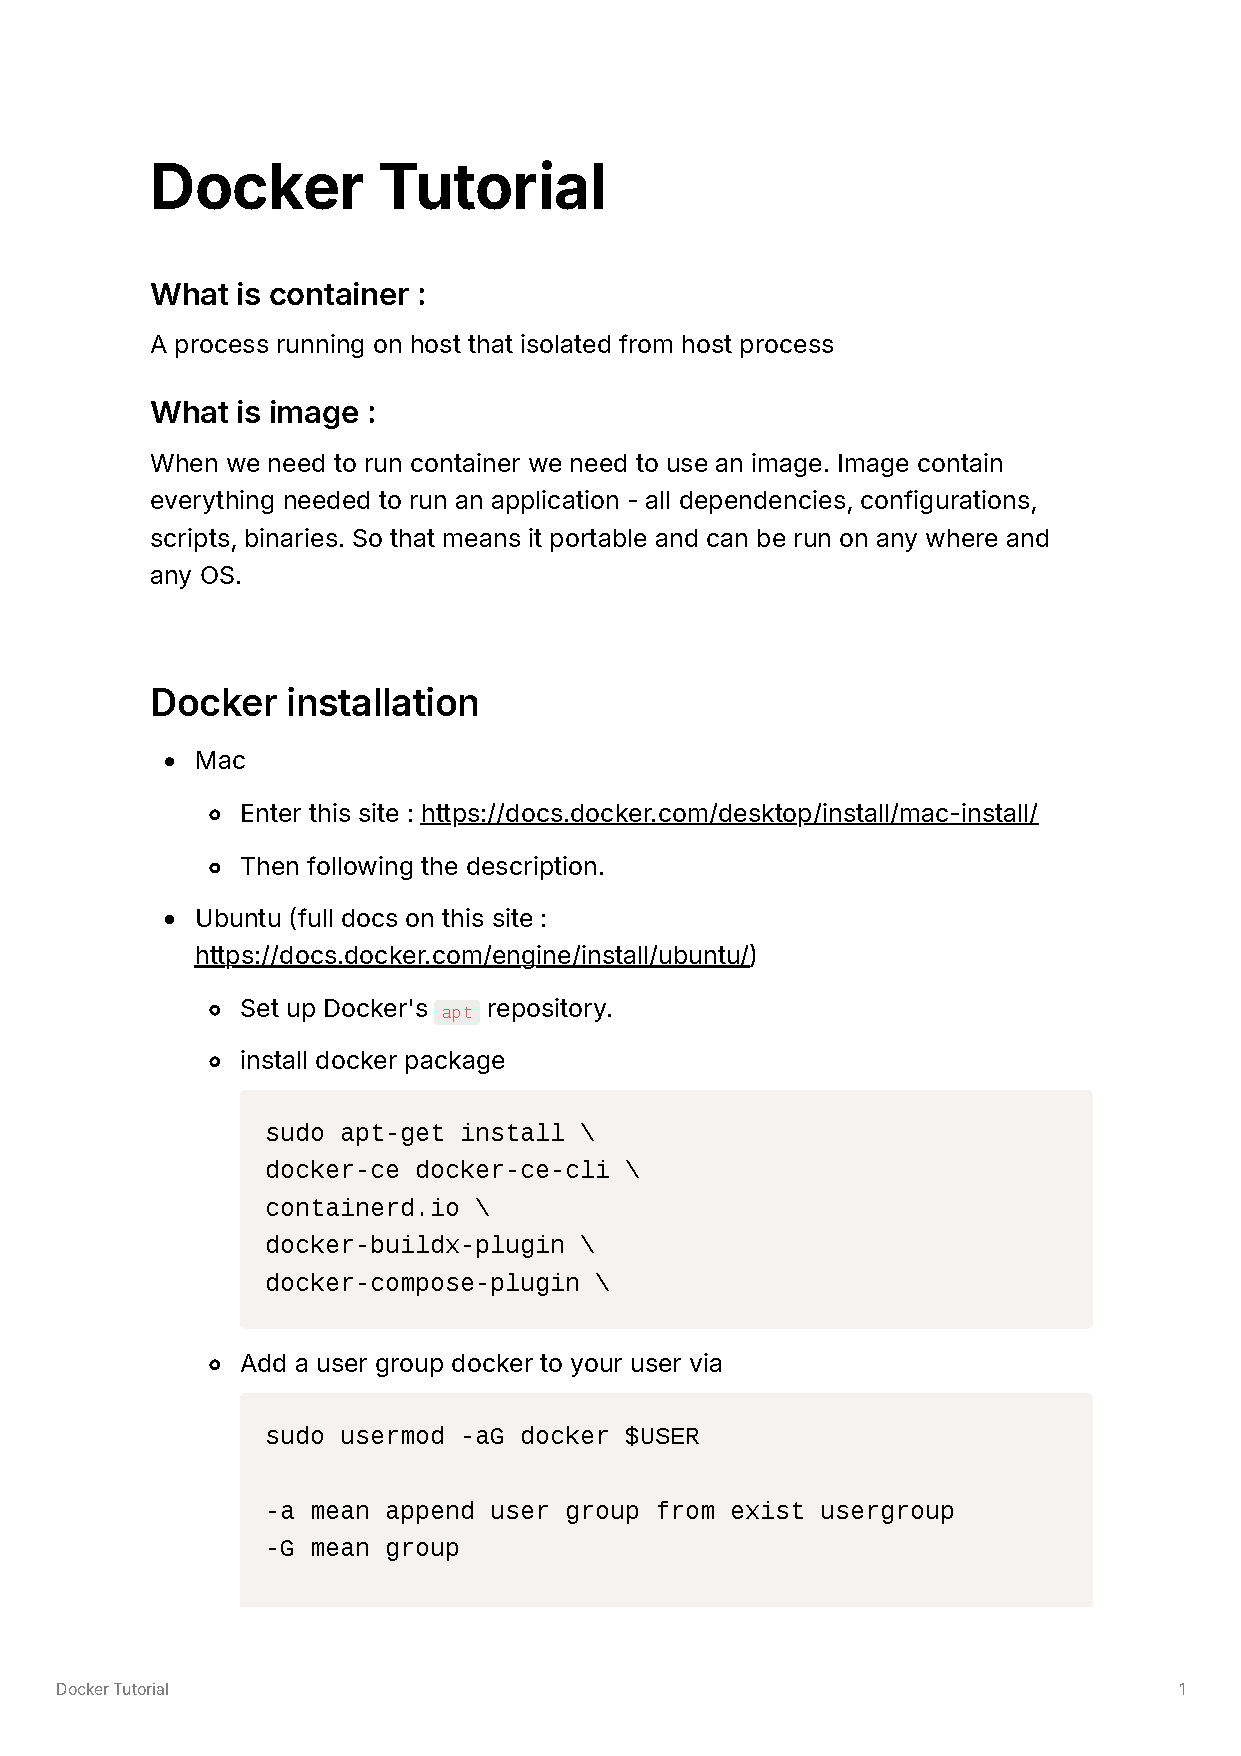
\includepdf[pages=-, scale=.8, pagecommand={\hypertarget{target:docker}{},\label{page:docker}}, nup=1x1, frame=true]{pdf/docker}
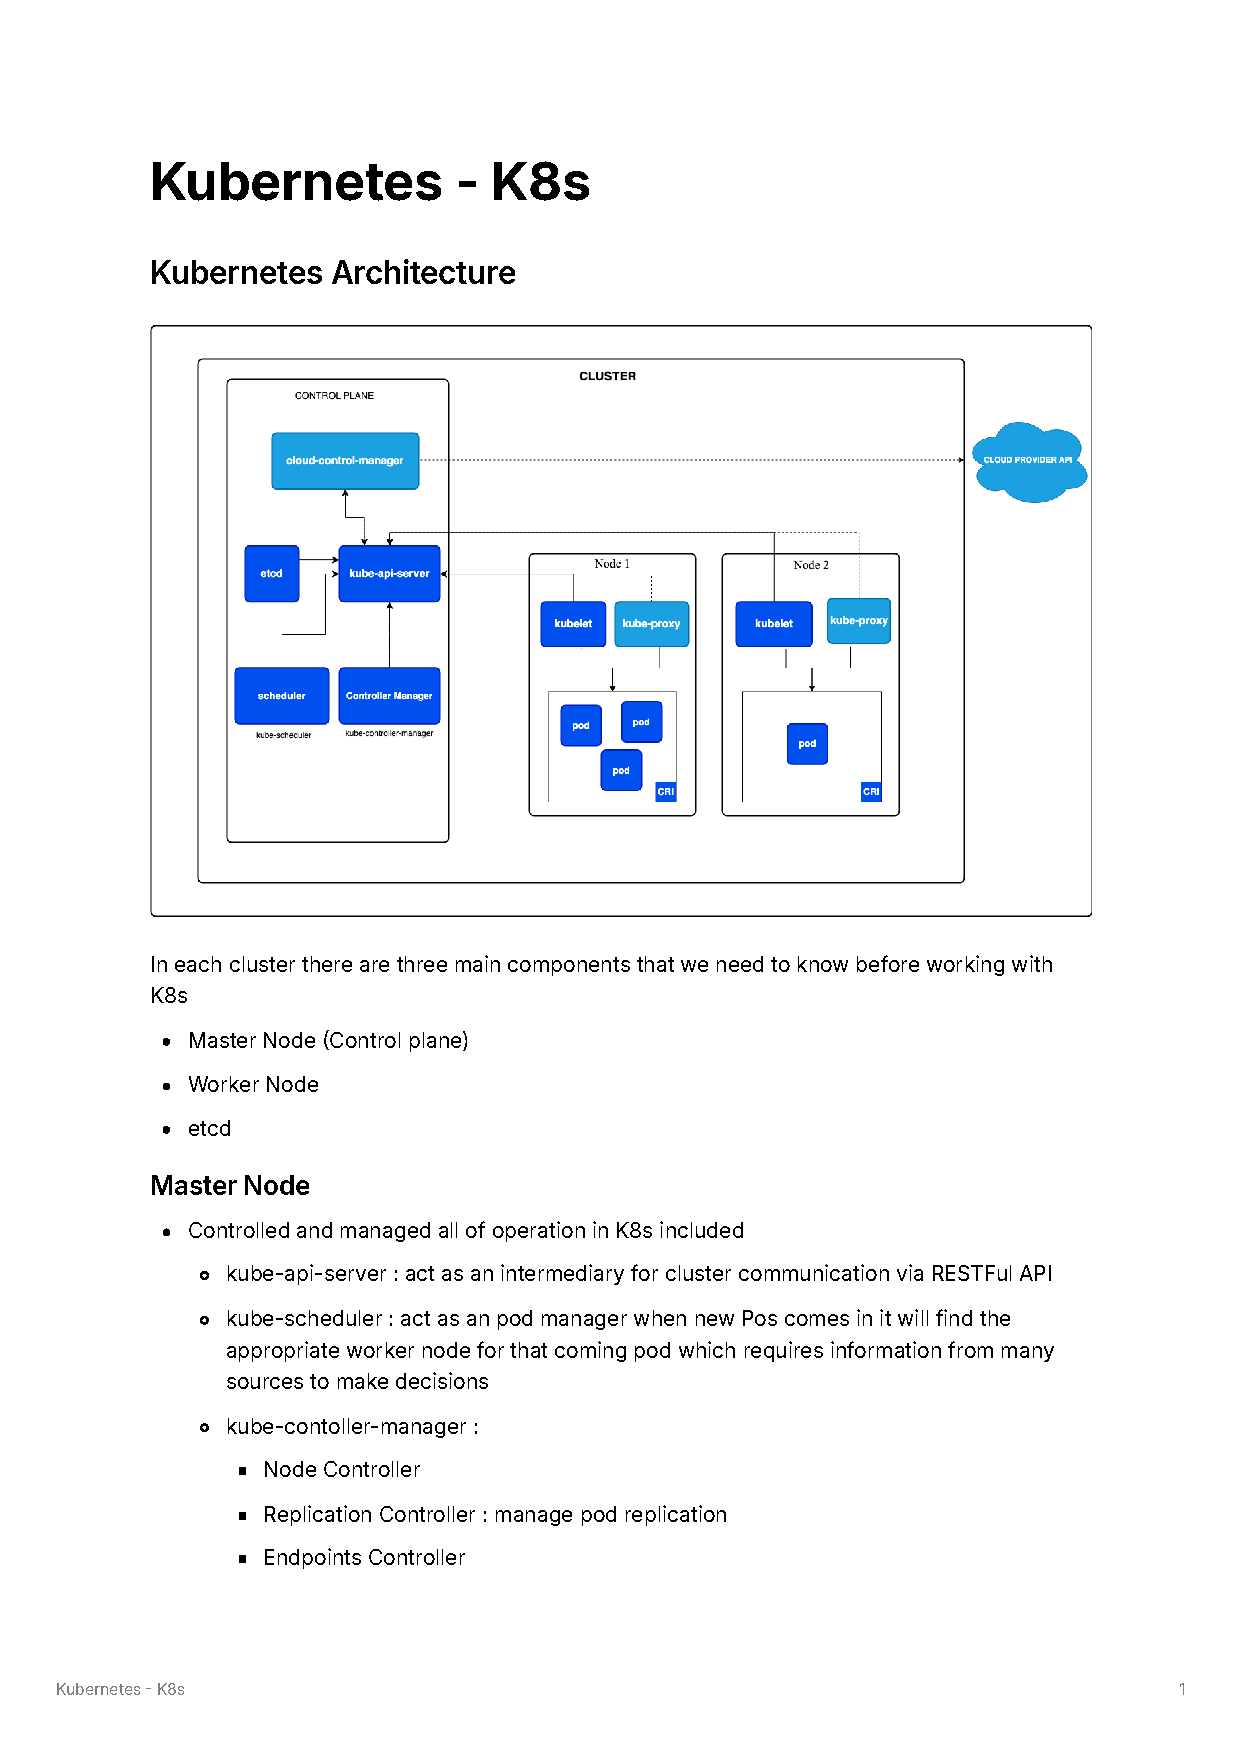
\includepdf[pages=-, scale=.8, pagecommand={\hypertarget{target:kube}{},\label{page:kube}}, nup=1x1, frame=true]{pdf/kube}
\includepdf[pages=-, scale=.8, pagecommand={\hypertarget{target:jenkins}{},\label{page:jenkins}}, nup=1x1, frame=true]{pdf/jenkins}
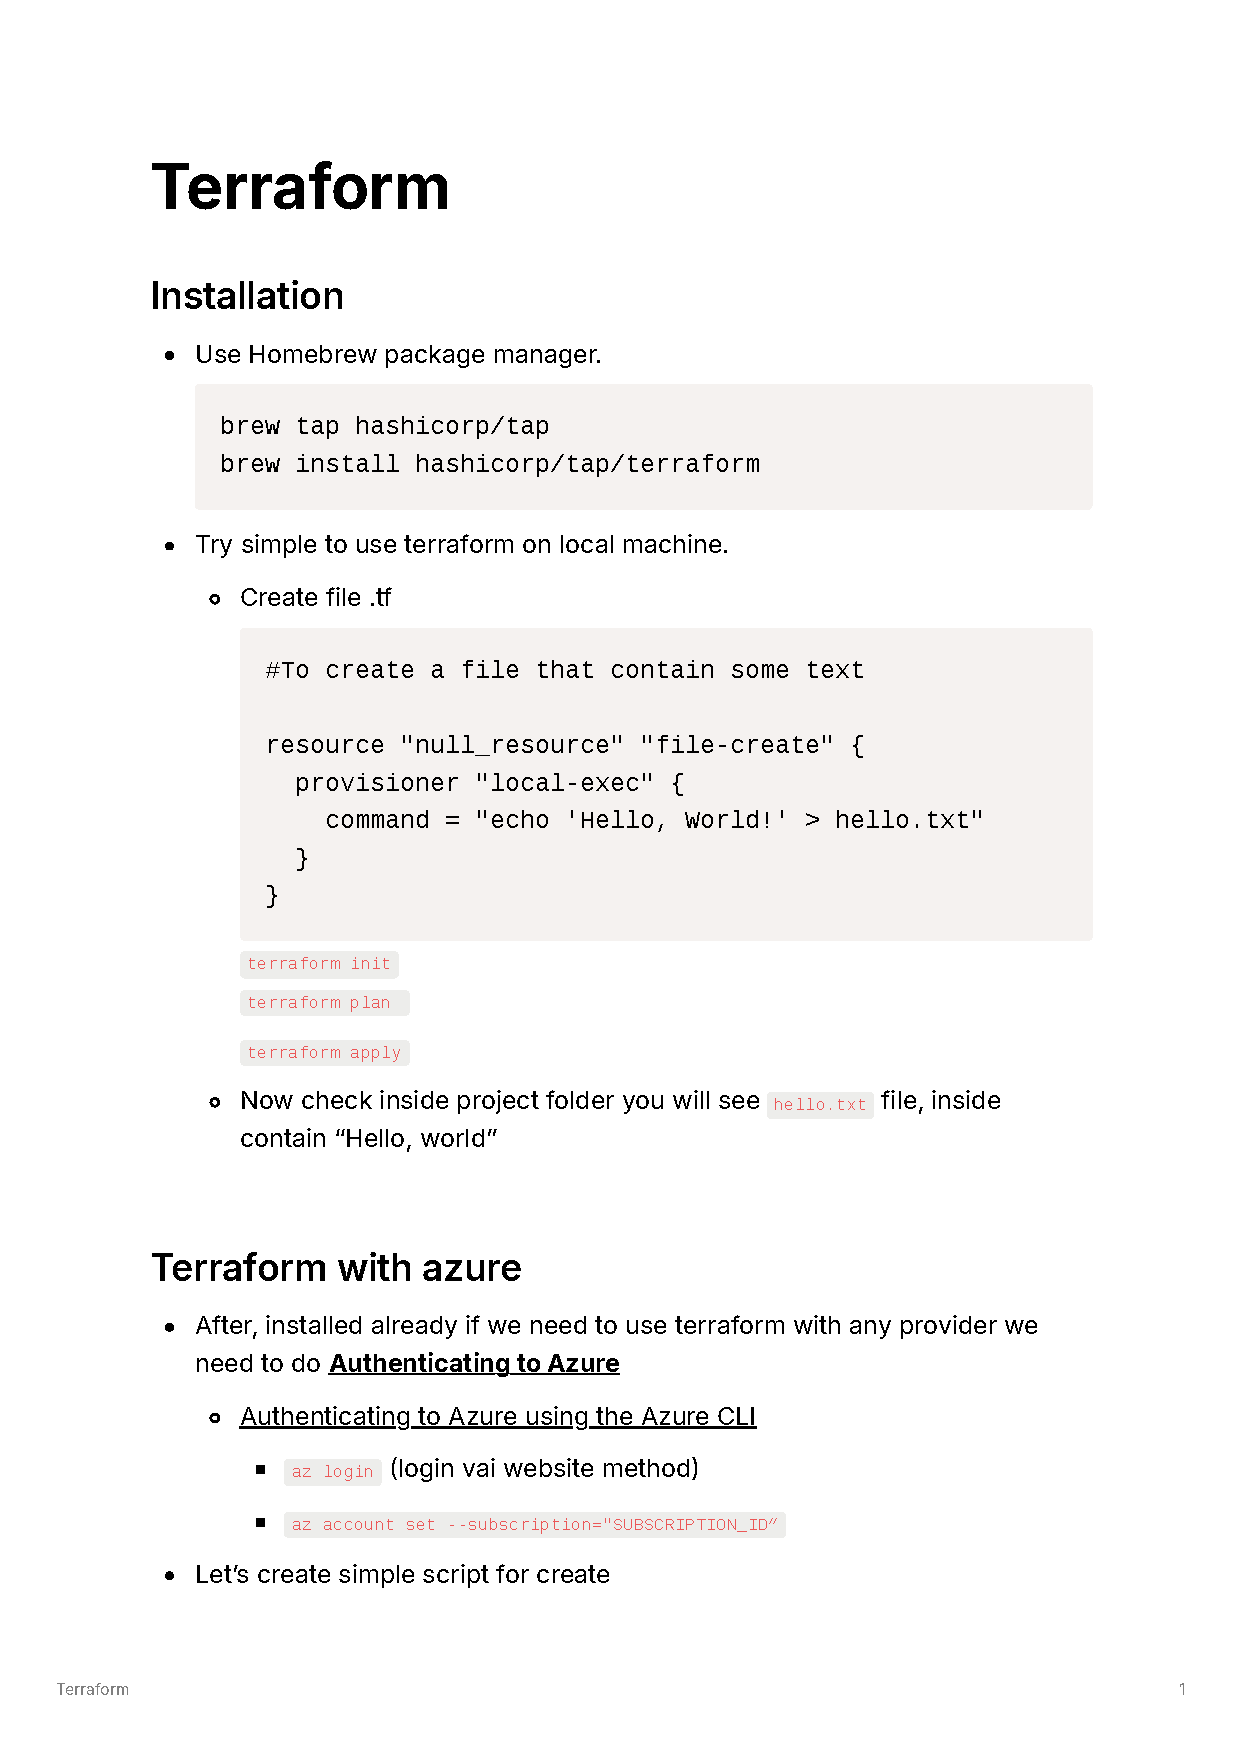
\includepdf[pages=-, scale=.8, pagecommand={\hypertarget{target:terraform}{},\label{page:terraform}}, nup=1x1, frame=true]{pdf/terraform}
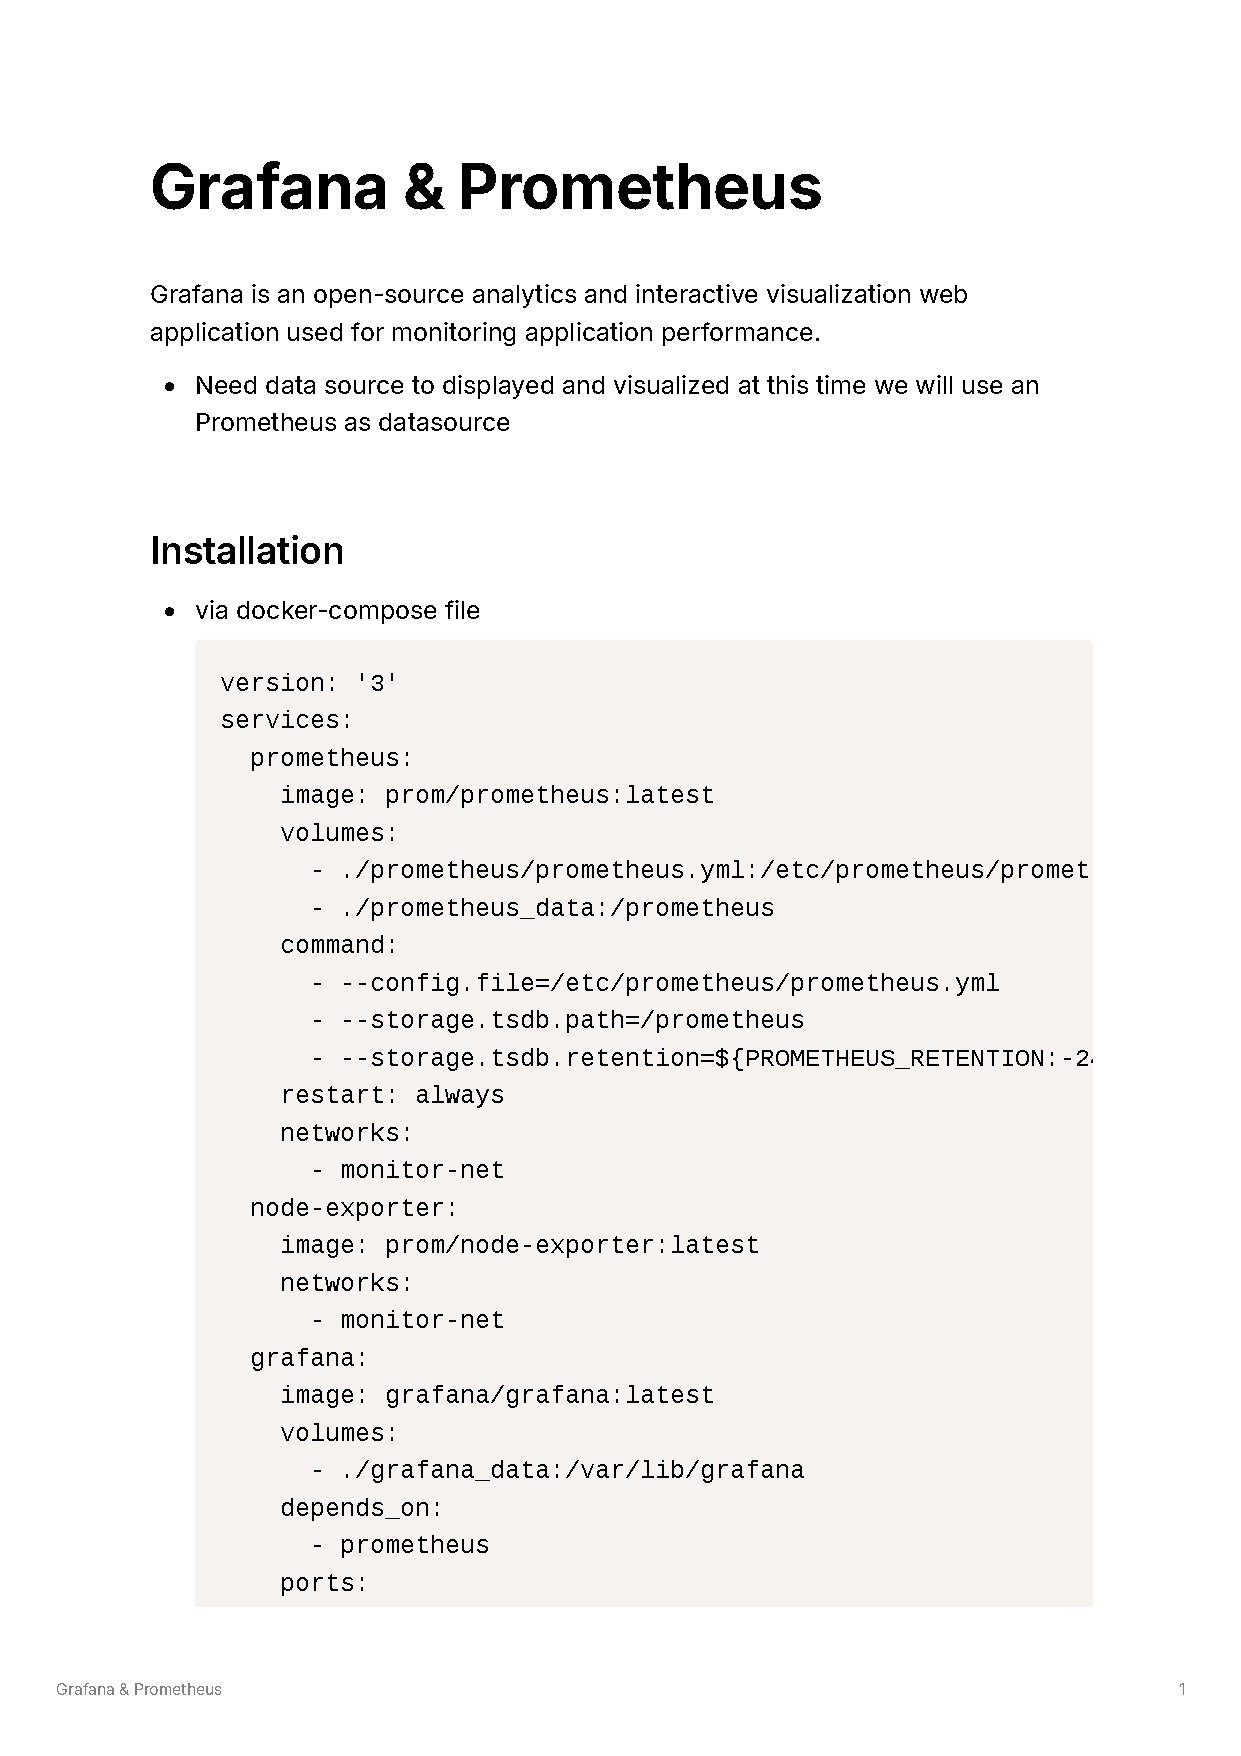
\includepdf[pages=-, scale=.8, pagecommand={\hypertarget{target:monitoring}{},\label{page:monitoring}}, nup=1x1, frame=true]{pdf/monitoring}
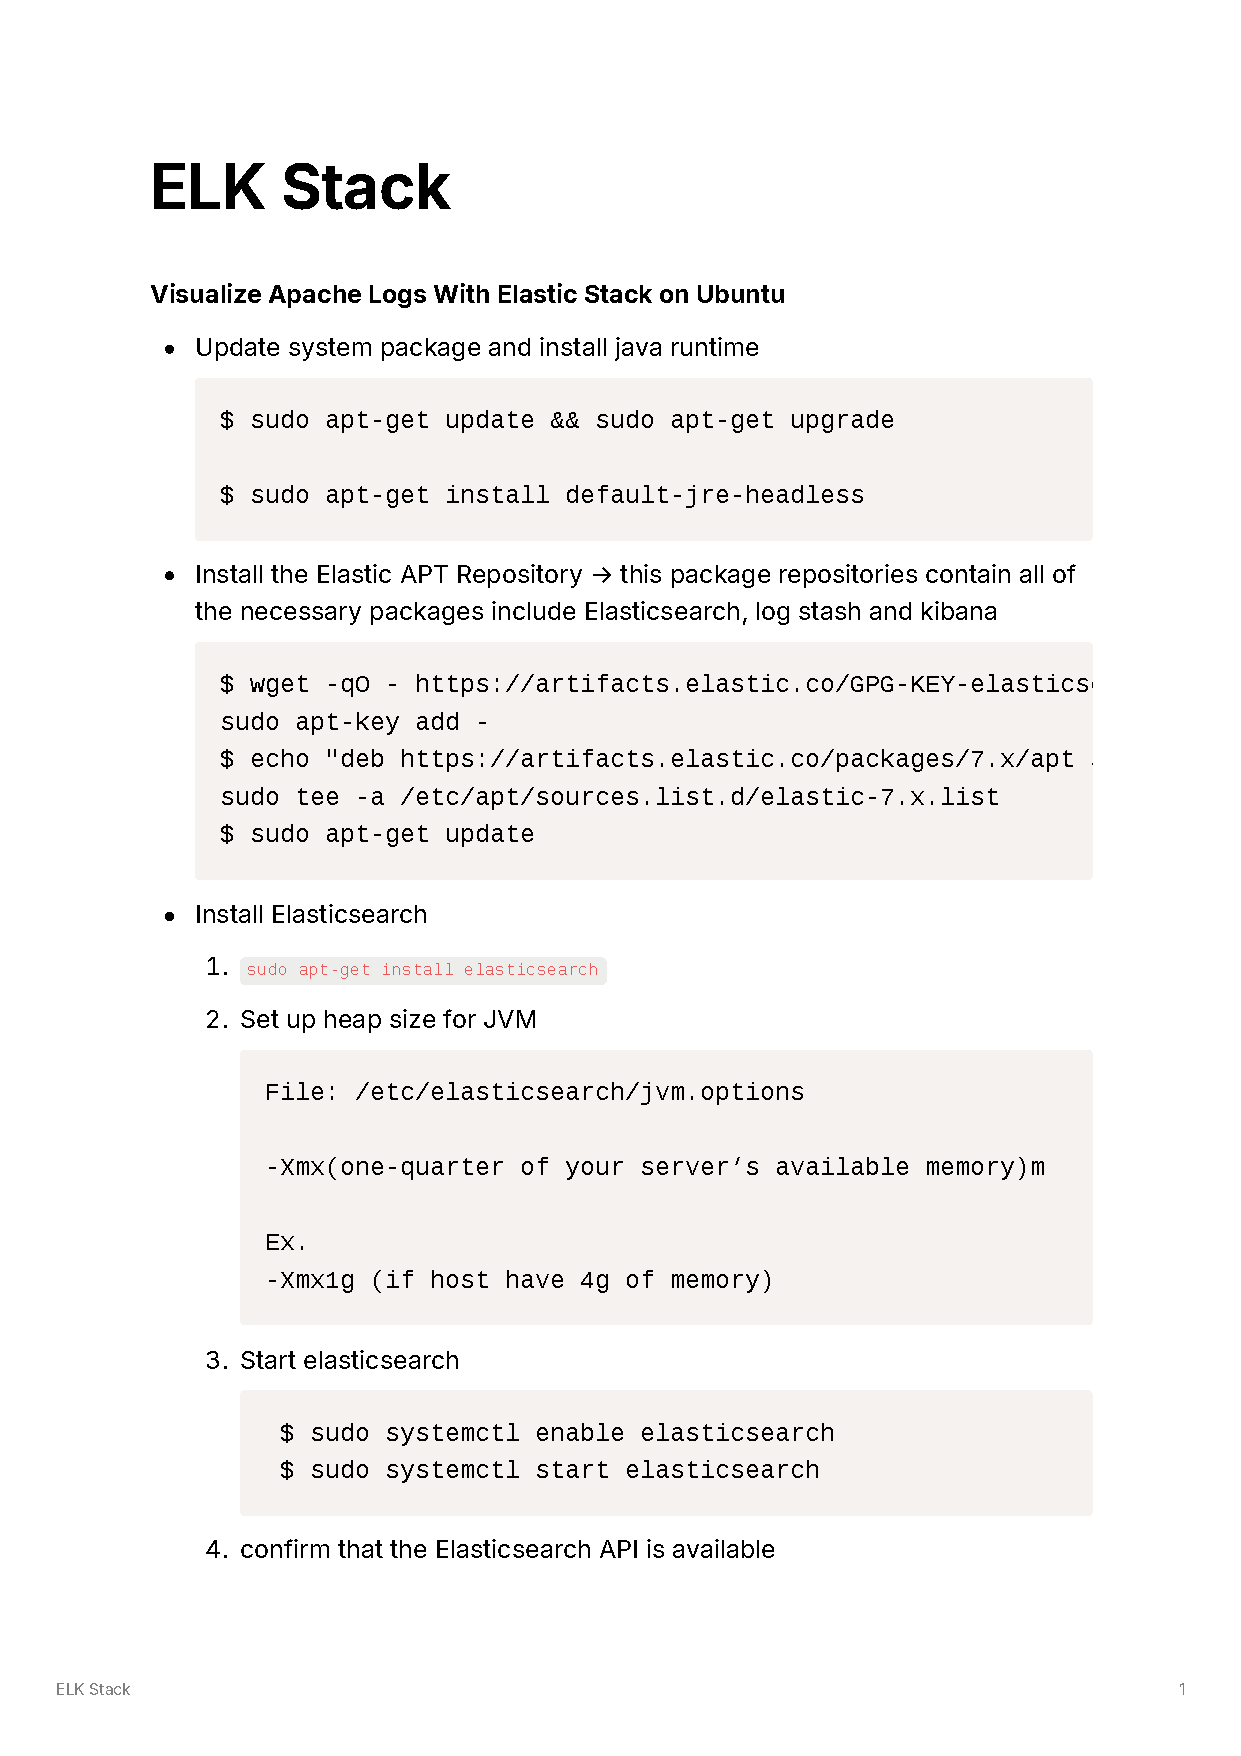
\includepdf[pages=-, scale=.8, pagecommand={\hypertarget{target:elk}{},\label{page:elk}}, nup=1x1, frame=true]{pdf/elk}